\section{Introduktion}\label{sec:introduktion}
Dette miniprojekt sigter mod at automatisere pointberegningen af afsluttede spilleplader i brætspillet King Domino. King Domino er et strategisk spil, hvor spillere bygger et grid på $5 \times 5$ dominobrikker bestående af forskellige terræntyper (bl.a. Forest, Field, Mine, Swamp, Lake og Grassland) og pointsamlende kroner.

Vores løsningsarkitektur deler opgaven op i tre specialiserede pipelines:
\begin{enumerate}
    \item \textbf{Machine Learning Pipeline:} En klassifikationsmodel, der ud fra farvedistributioner og træk identificerer terræntypen for de 25 individuelle felter på spillepladen.
    \item \textbf{Computer Vision Pipeline:} En template-matching algoritme, som lokaliserer og tæller antallet af pointgivende kroner.
    \item \textbf{Algoritmisk Pipeline:} Et nabo-søgende regelsæt (Flood-fill), der samler ens terræner i lukkede områder (clusters) og udfører den underliggende matematik for spillets pointfordeling.
\end{enumerate}

I det følgende gennemgås de implementerede metoder, de tekniske samt matematiske valg der ligger til grund for systemets udvikling, og endeligt en refleksion over mødte udfordringer under udviklingen af systemet.

% --- BILLEDE 1: Systemarkitektur / Overordnet flow ---
\begin{figure}[htbp]
    \centering
    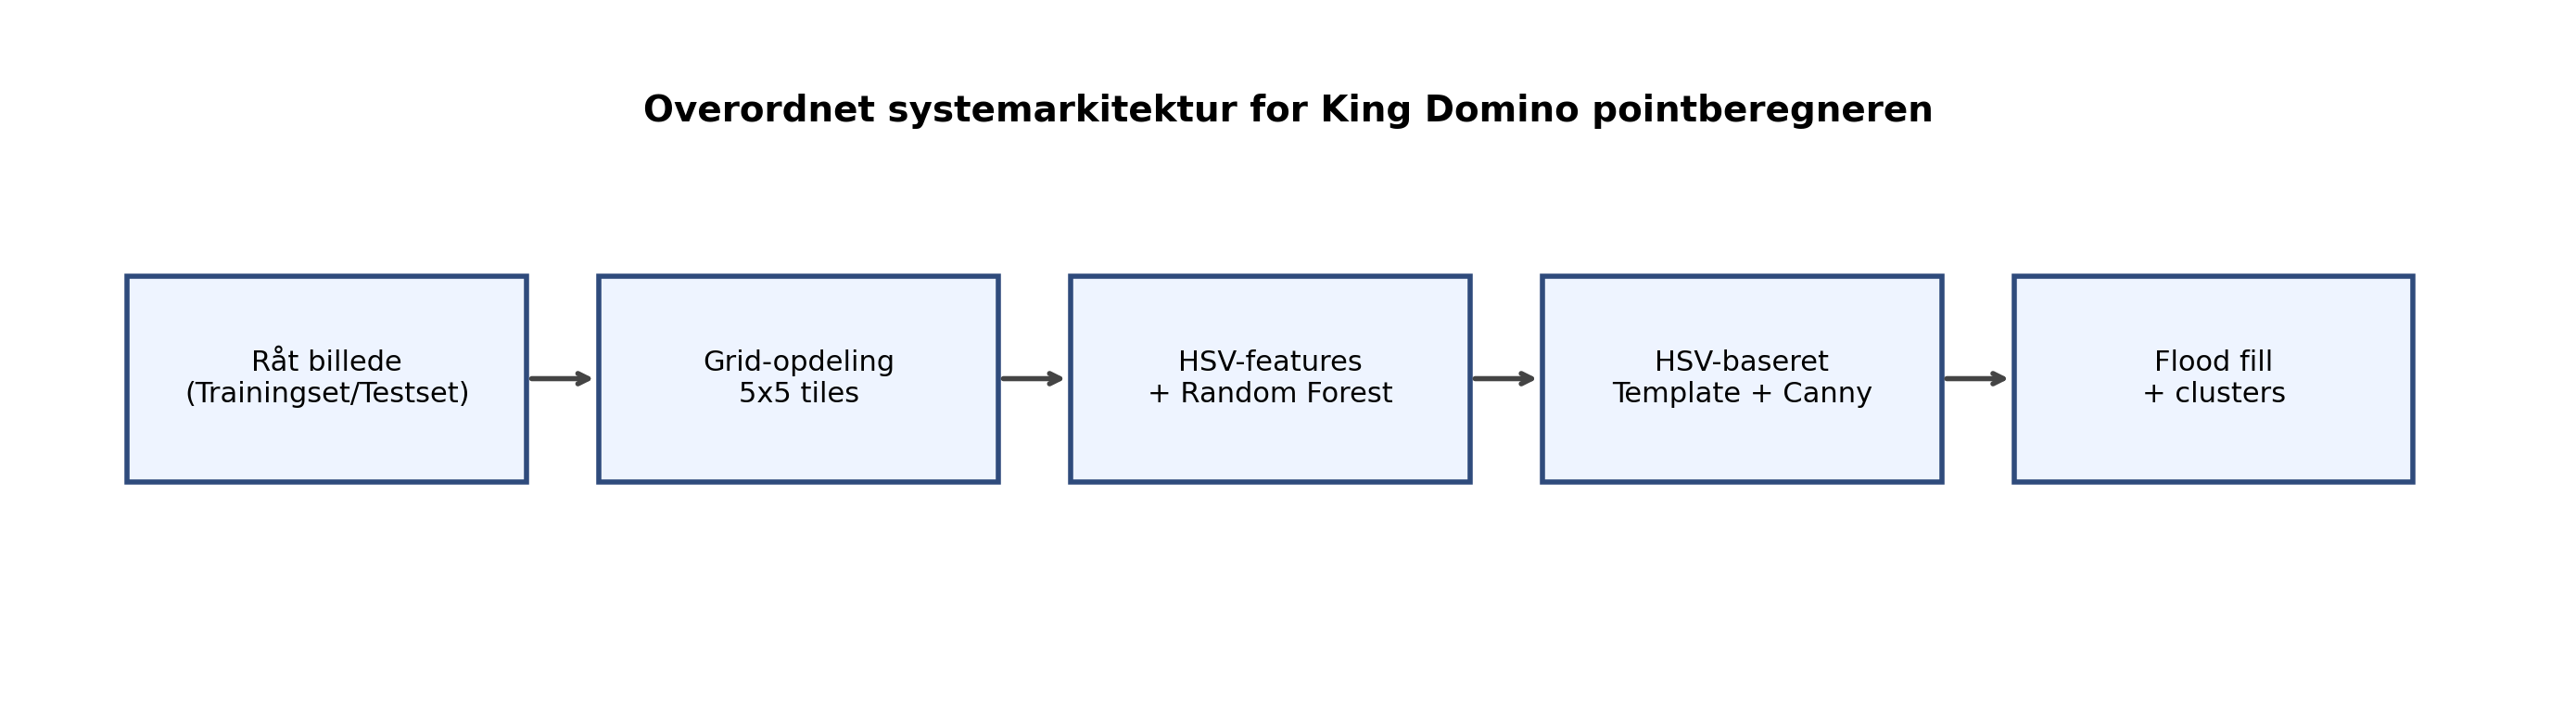
\includegraphics[width=0.88\textwidth]{figures/systemarkitektur.png}
    \caption{Overordnet systemarkitektur for King Domino pointberegneren, der viser flowet fra råt billede til endelig score.}
    \label{fig:arkitektur}
\end{figure}

Figur~\ref{fig:arkitektur} illustrerer den fulde behandlingskæde i systemet. Pipeline-opdelingen gør det muligt at fejlsøge modulært, så fejl i samlet score kan isoleres til enten terrænklassificering, krone-detektion eller selve pointberegningen.

\section{Implementering}\label{sec:implementering}

\subsection{Databehandling og Feature Extraction}
For at maskinesystemet kan håndtere de rå spilleplader, isoleres hvert af spillepladens felter matematisk i et 2D grid på $5 \times 5$ felter. Systemet skærer systematisk det totale billede op i rektangulære \textit{tiles} via list slicing (eksempelvis \texttt{image[y*100 : (y+1)*100, ...]}).

Hvert felt konverteres fra standard BGR (Blå, Grøn, Rød) til HSV (Hue, Saturation, Value) farverummet. Denne konvertering er udvalgt pga. dens robusthed overfor varierende lysforhold og skygger, som ellers kan manipulere med RGB-værdierne.

For at formidle feltets egenskaber struktureret til den efterfølgende machine learning-model, genereres en feature-vektor ud fra de tre HSV kanaler. Der udtages median-værdien for hvert spektrum:

$$
\text{Med-Værdier} = \{H_{\text{median}}, S_{\text{median}}, V_{\text{median}}\}
$$

Dernæst trækkes der histogramegenskaber, hvor farvernes fordeling inddeles i intervaller (bins) af størrelsen 10. \texttt{Hue}-kanalen fordeles på intervaller fra 0-180, mens \texttt{Saturation} og \texttt{Value} indeholder fordelinger af værdierne 0-255. Denne matematisk nedbrudte profilering genererer en dataset-række med i alt 74 detaljerede features pr. felt, som danner det statistiske fundament for genkendelsessystemet.

% --- BILLEDE 2: Grid-udklip og feature-visualisering ---
\begin{figure}[htbp]
    \centering
    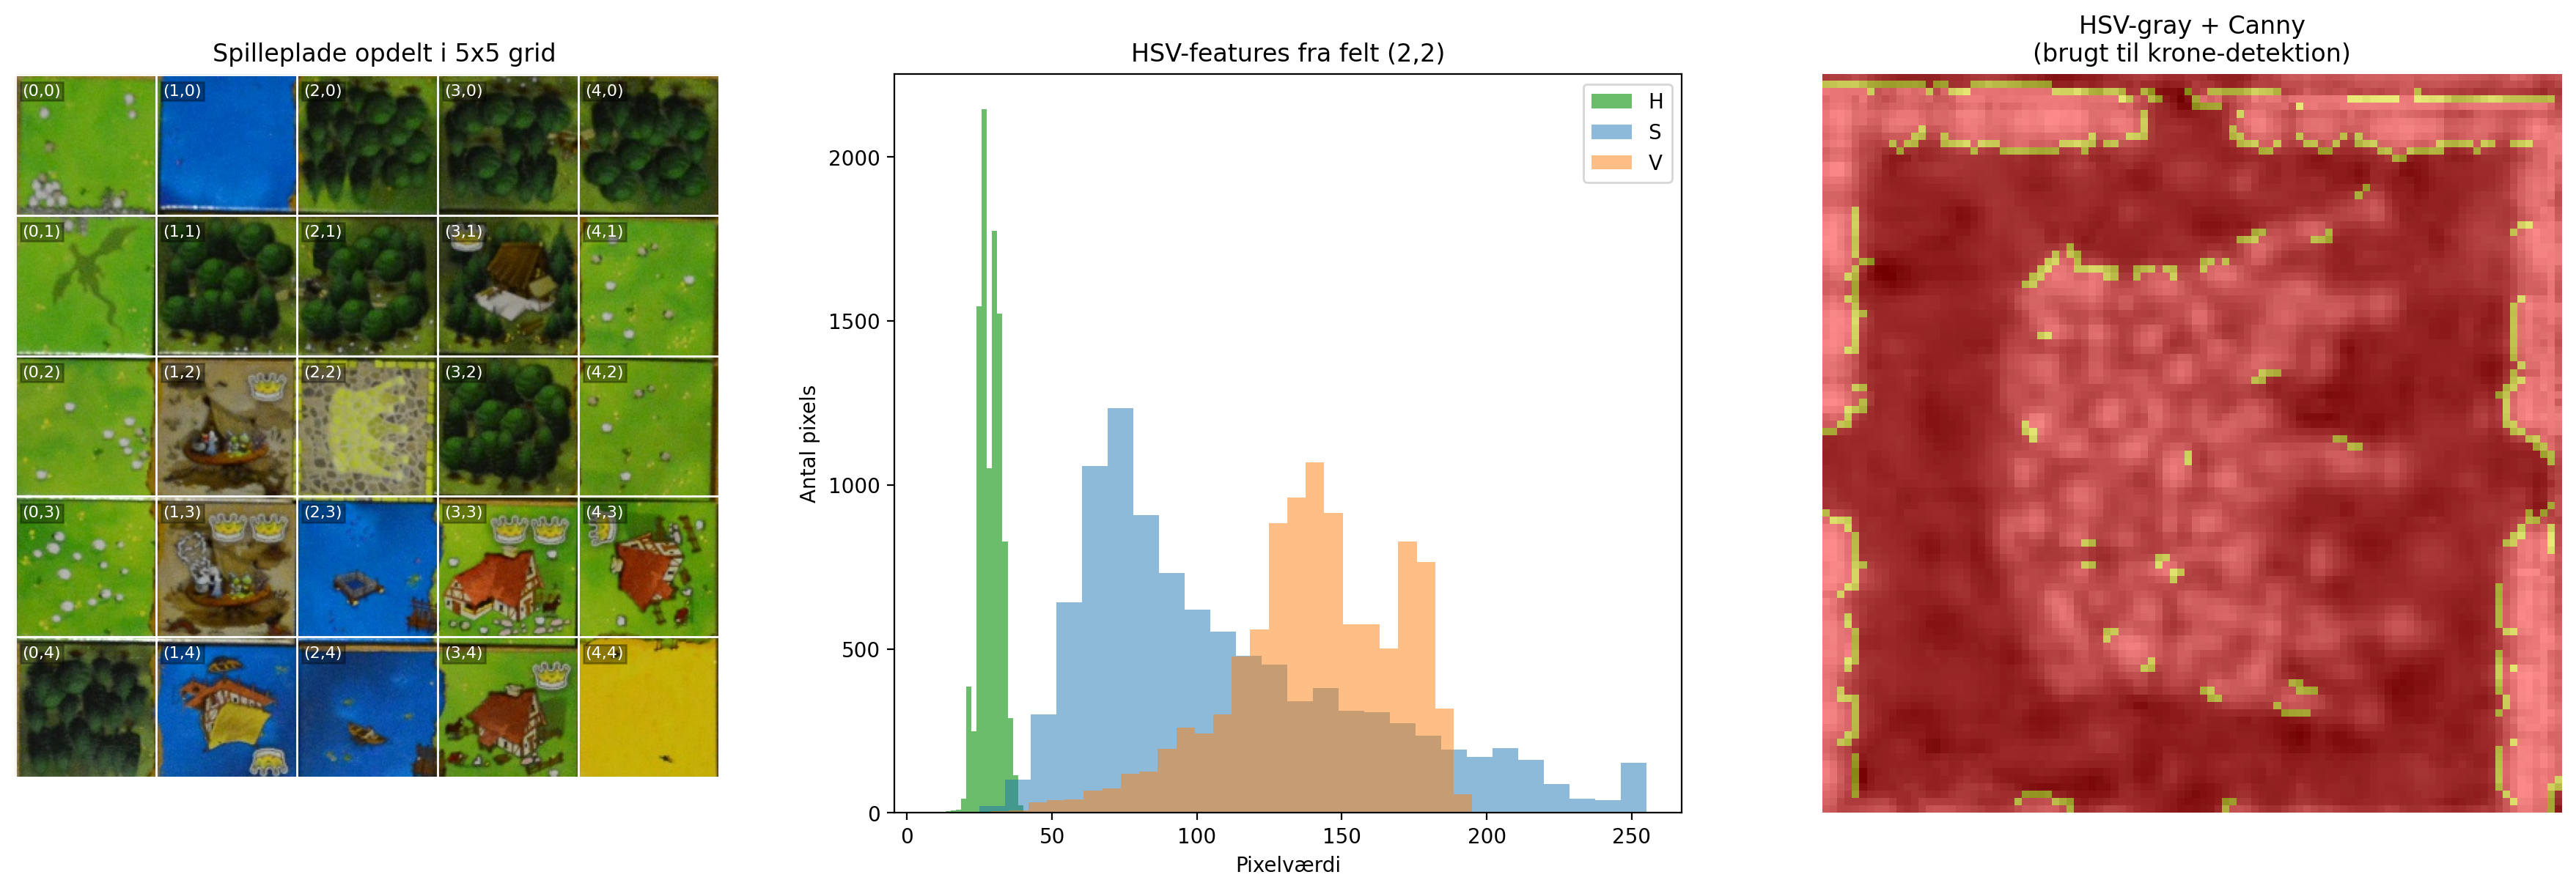
\includegraphics[width=0.95\textwidth]{figures/grid_feature_visualization.png}
    \caption{Et eksempel på en spilleplade opdelt i $5 \times 5$ grid, samt visualisering af både HSV-features (terrænklassificering) og HSV-gray/Canny-features (krone-detektion) fra et enkelt felt.}
    \label{fig:grid_extraction}
\end{figure}

Figur~\ref{fig:grid_extraction} viser, at systemet bruger forskellige feature-repræsentationer til forskellige delopgaver: HSV-histogrammer til terrænklassificering og en HSV-baseret gråtoneprojektion med Canny-kanter til krone-detektion. Formålet er at vælge den repræsentation, der bedst understøtter den konkrete beslutning i hvert modul.

\subsection{Machine Learning: Terrænklassificering}
Til klassificeringen af de seks generiske terræntyper samt den farveløse \texttt{blank}-type fungerer en \textit{Random Forest Classifier} model som grundsten. Modellen er trænet på manuelle annotationer i tilhørende træningssæt via \texttt{LabelEncoder}, som tillader algoritmen at arbejde kvantitativt med tekst-strenge.

Random Forest-modellen er initieret med 100 individuelle beslutningstræer (estimators) og et \texttt{min\_samples\_split} på 10. Valget af Random Forest er understøttet af metodens udtalte styrke indenfor tabulær feature-data; den kan tildele stor vægt til vigtige features (eksempelvis tilstedeværelsen af højt udslag i grønne H-bins ved skov- og græsfelter), men tillader en samlet og udjævnet afstemning blandt de 100 træer, hvilket minimerer risikoen for ren overfitting på det begrænsede King Domino test- og træningsdata.

\subsection{Computer Vision: Krone-detektion}
Lokaliseringen af kroner præsenterer en markant skalering- og rotationsudfordring, idet spilbrikkerne kan roteres i flere retninger af spillerne. Kronedetektionen løses gennem metoden \textit{Normeret Krydskorrelation} (Normed Cross-Correlation) indenfor området Template Matching (\texttt{cv.TM\_CCOEFF\_NORMED}). I den endelige implementation udføres søgningen på hele spillepladen i HSV-farverummet, hvorefter verificering sker med Canny-kantinformation fra en HSV-baseret gråtoneprojektion.

Flere formskabeloner af spillets point-kroner (med forskellige baggrunde) filtreres systematisk mod hele pladen med template-specifikke tærskler. For at opnå rotation- og skalarobusthed itereres der over vinklerne $\theta = \{0^\circ, 90^\circ, 180^\circ, 270^\circ\}$ samt en smal skaleringsinterval omkring den forventede størrelse.

Efter første template-match anvender systemet Canny Edge-verifikation, så falske positive kandidater kan frasorteres ved at sammenligne konturer fremfor kun rå pixelkorrelation. De endelige kroner projiceres derefter tilbage til de enkelte felter ved hjælp af detekterede bounding box-centre.

Resultater samles af algoritmen via \texttt{cv.groupRectangles}, hvilket konsoliderer overlap og reducerer duplikerede detektioner. Denne post-processing er central for en stabil kroneoptælling per felt.

% --- BILLEDE 3: Template Matching processen ---
\begin{figure}[htbp]
    \centering
    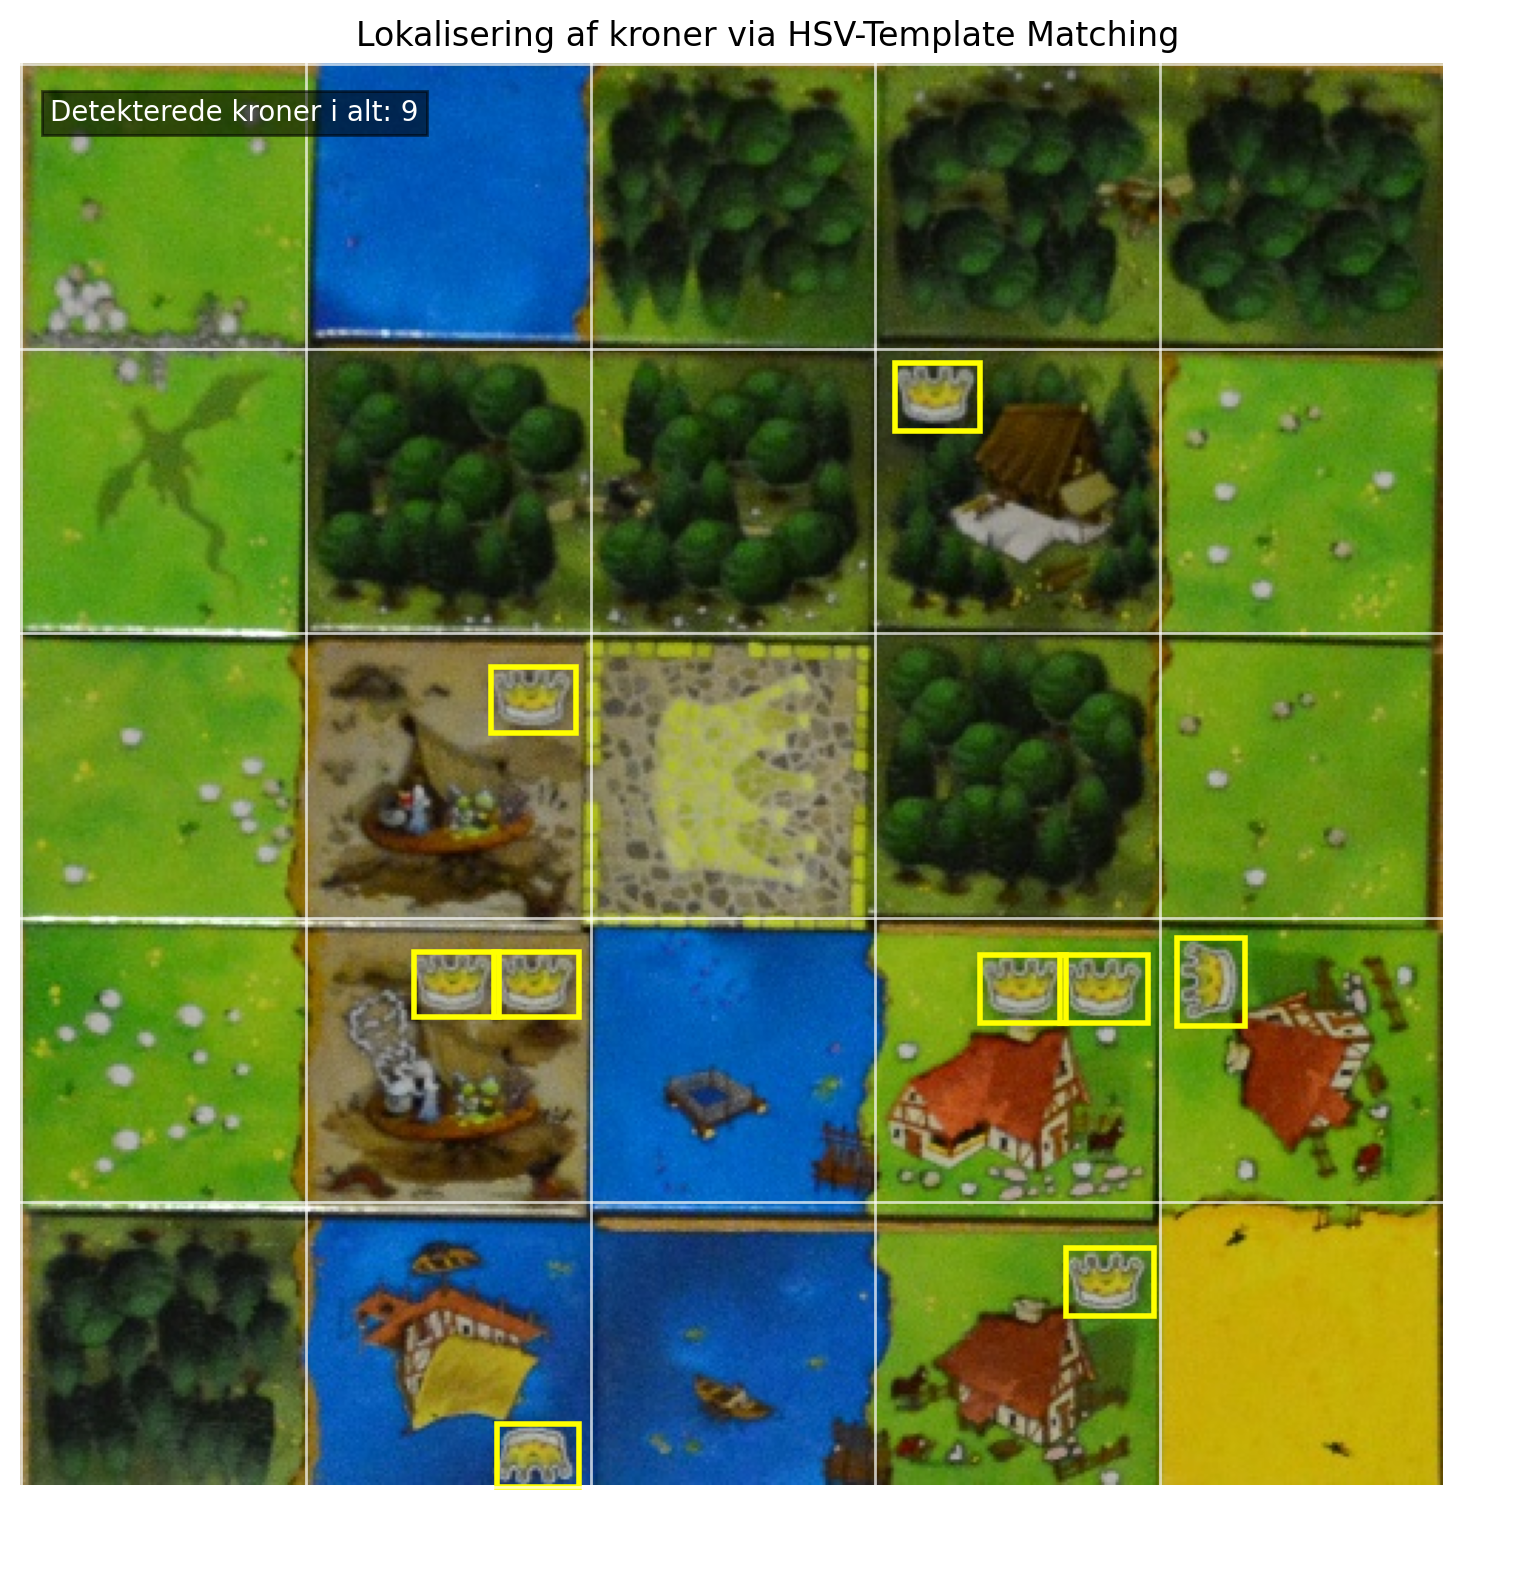
\includegraphics[width=0.85\textwidth]{figures/template_matching.png}
    \caption{Lokalisering af kroner via Template Matching og efterfølgende verifikation. Figuren kan vise rotation, skalering og den endelige markering af detekterede kroner.}
    \label{fig:templatematching}
\end{figure}

I Figur~\ref{fig:templatematching} vises de endelige detektioner efter filtrering. Figuren skal læses sammen med den efterfølgende debug-figur, hvor forskellen mellem rå matches og verificerede matches tydeliggøres.

\begin{figure}[htbp]
    \centering
    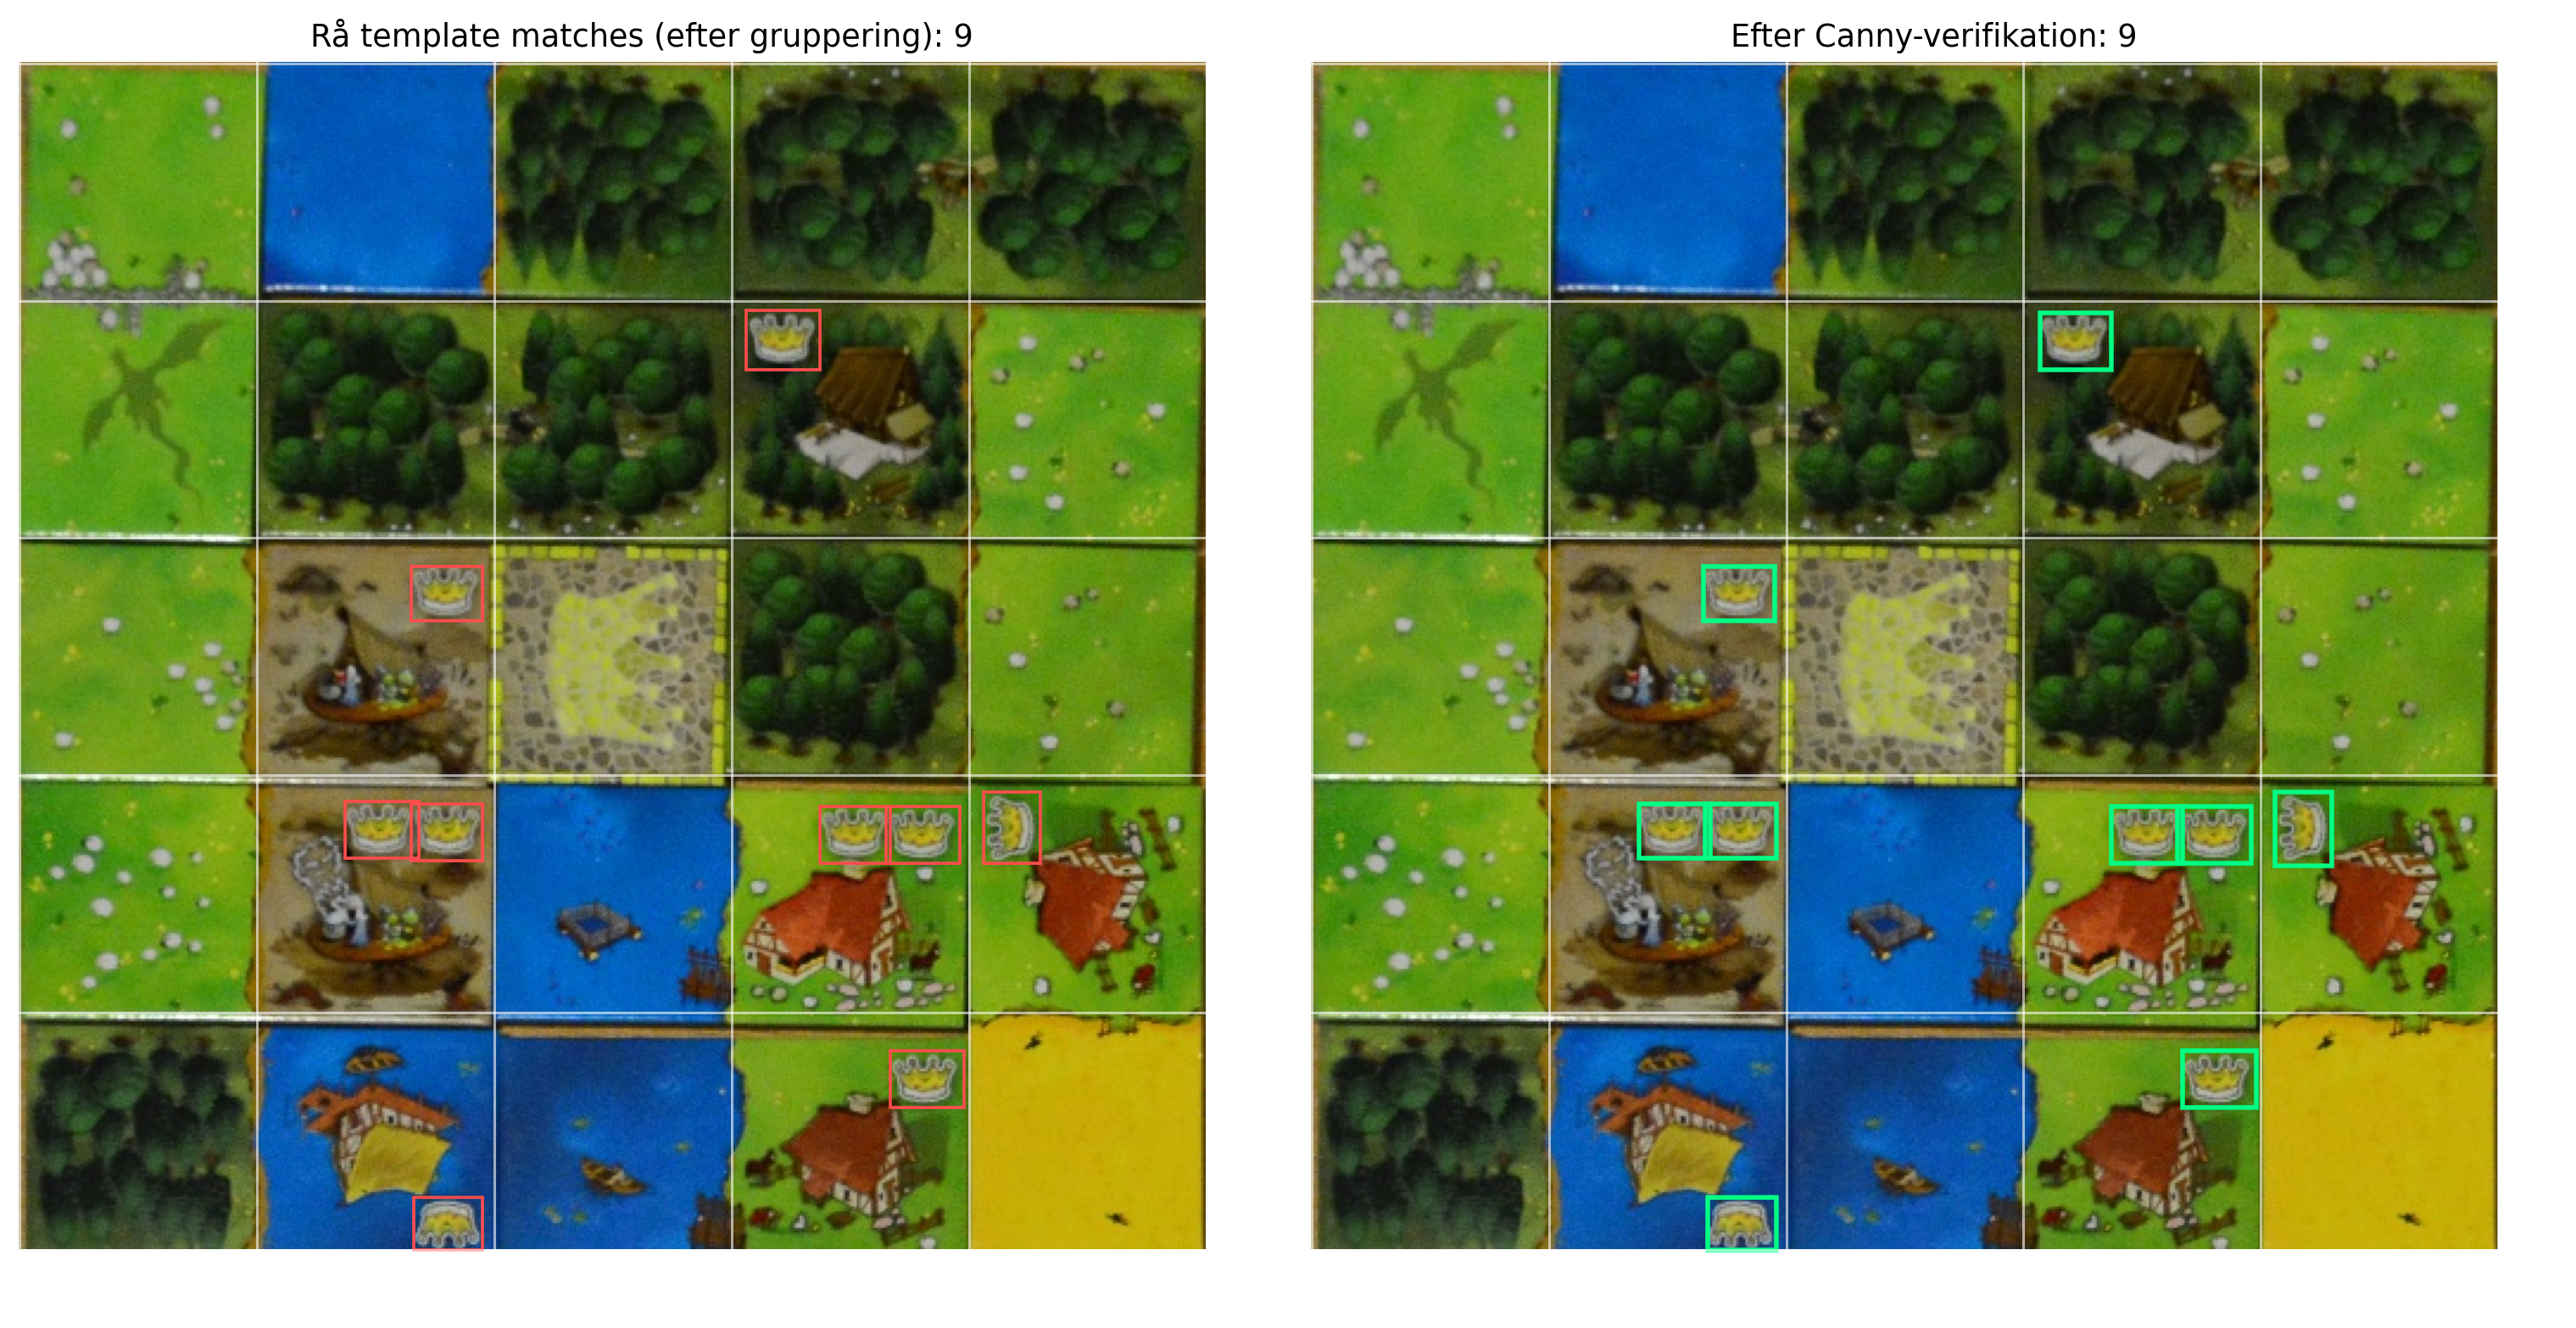
\includegraphics[width=0.98\textwidth]{figures/template_matching_debug.png}
    \caption{Side-by-side sammenligning af rå template matches (venstre) og matches efter Canny-verifikation (højre). Figuren forklarer, hvorfor nogle kandidater filtreres væk i den endelige kroneoptælling.}
    \label{fig:templatematching_debug}
\end{figure}

Figur~\ref{fig:templatematching_debug} fungerer som metodevalidering: venstre panel viser alle kandidater fundet af template matching-trinnet, mens højre panel viser de kandidater, der overlever konturkontrollen. Dermed dokumenteres det, at manglende kroner i output ikke er en visualiseringsfejl, men en konsekvens af de valgte tærskler og verifikationskrav.

\subsection{Algoritmik: Pointberegnings logik}
Sidste trin af opgaven varetages af det specialudviklede Point Calculator modul, hvilket evaluerer hele spillepladens $5 \times 5$ grid i samklang. Modulets funktion er at bygge \textit{clusters}, hvor identiske og tilstødende terræntyper grupperes i henhold til spillets love.

Her implementeres en list-baseret \texttt{Flood Fill}-algoritme, der identificerer naboceller alene via vertikale og horisontale offsets ($x\pm 1, y$ og $x, y\pm 1$). Diagonale offsets ($dx=\pm 1, dy=\pm 1$) er bevidst ekskluderet i henhold til de officielle King Domino spilleregler.

Hvert identificeret terræn forbliver ubesøgt indtil en nabosøgning igangsættes, hvori enhver korrekt nabo tilføjes felt-længden ($T_c$) og arver evt. kroneværdi ($K_c$) i dette lukkede område $c$. Derved danner den bagvedliggende pointmatematik spillets score:

$$
\text{Total Score} = \sum_{c \in \text{Clusters}} \left( T_c \times K_c \right)
$$

Logikken leverer derved det samlede slutresultat samt returnerer fuldt regnskab for de gennemsøgte zoner, en feature specielt designet for manuel transparens og debugging af systemet.

% --- BILLEDE 4: Flood Fill / Cluster visualisering ---
\begin{figure}[htbp]
    \centering
    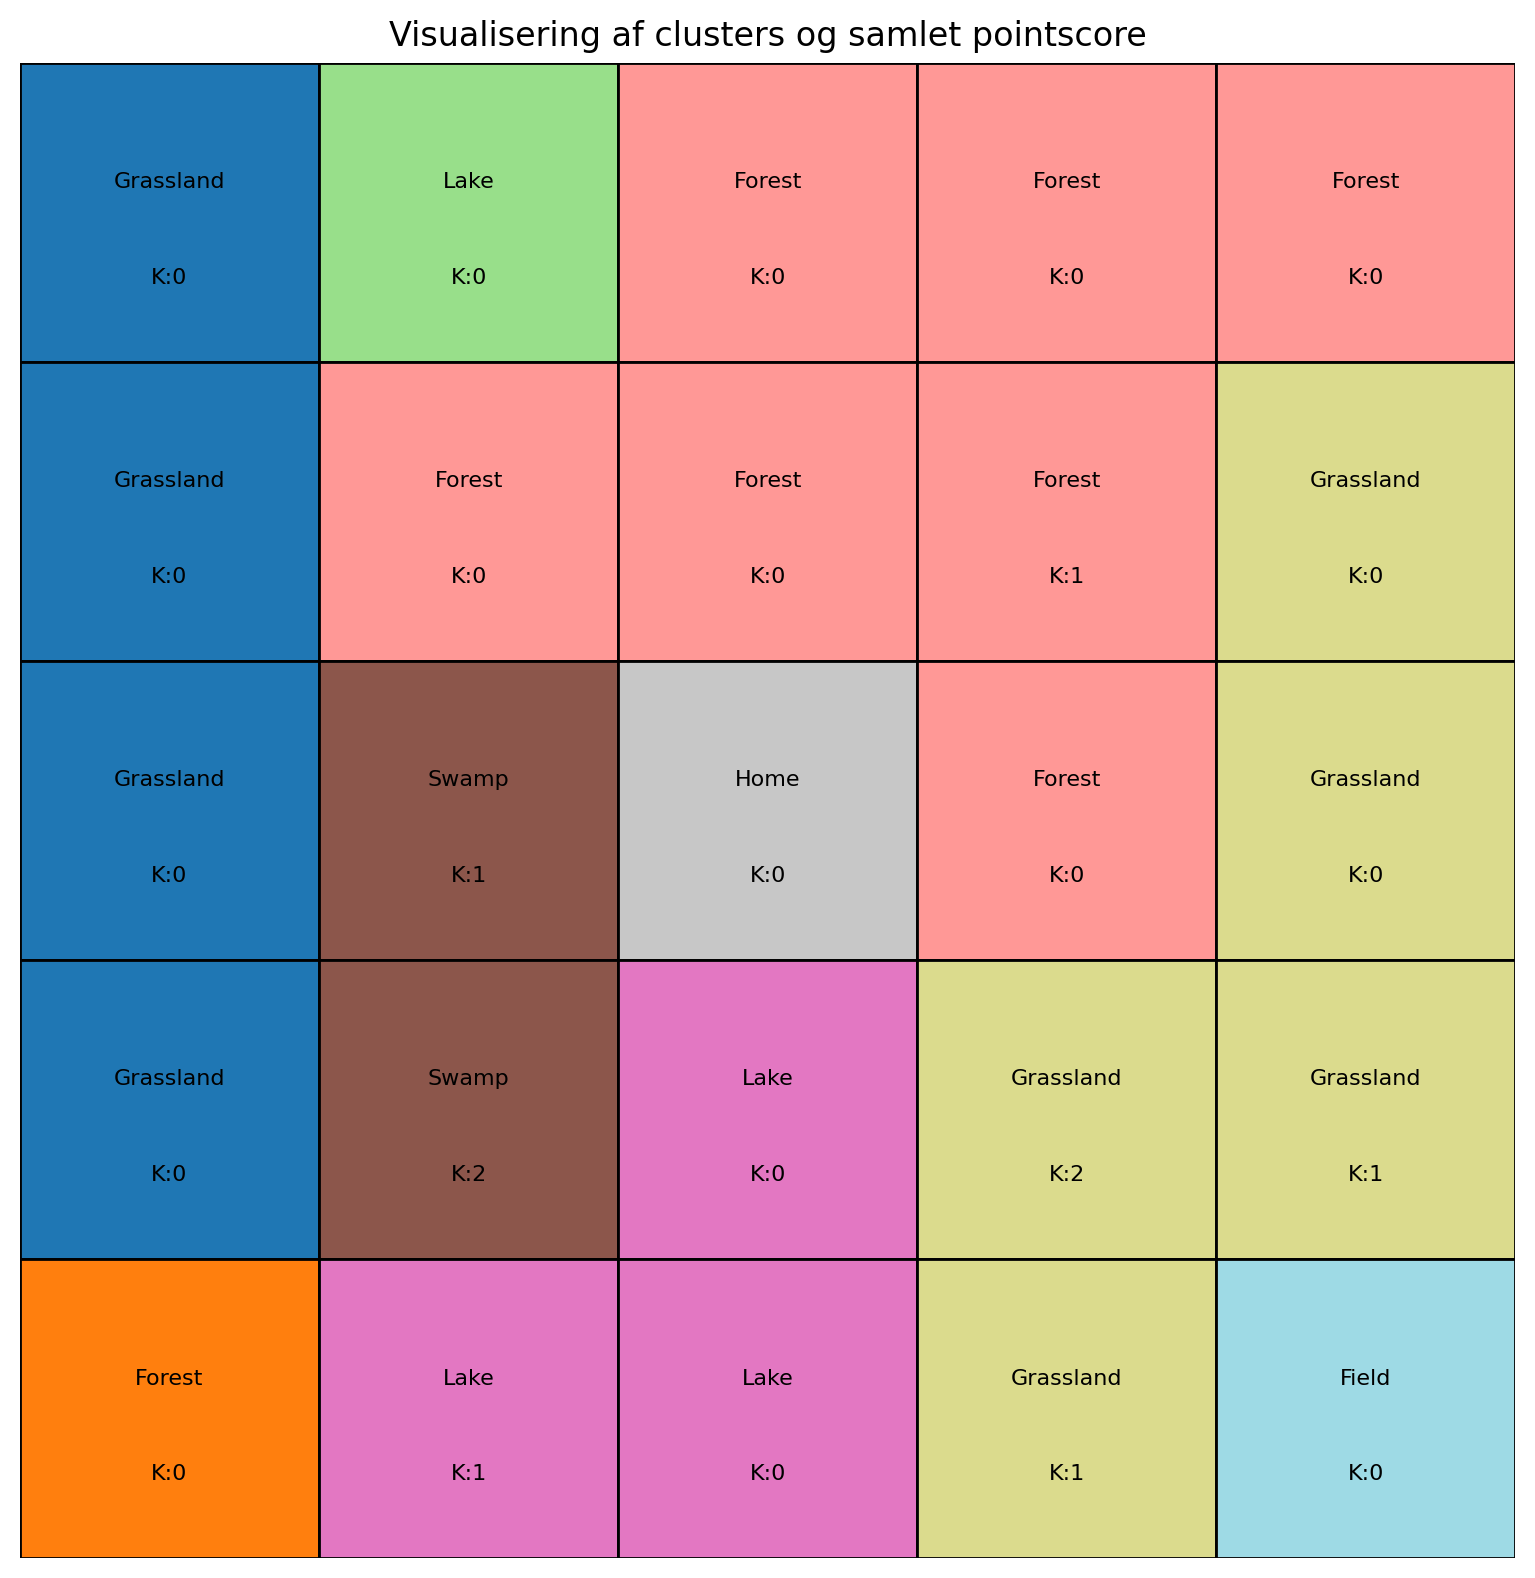
\includegraphics[width=0.9\textwidth]{figures/floodfill_resultat.png}
    \caption{Visualisering af lukkede områder (clusters) fundet via Flood Fill, samt beregningen af den samlede pointscore for pladen.}
    \label{fig:floodfill}
\end{figure}

Figur~\ref{fig:floodfill} viser den direkte kobling mellem cluster-fund og pointsum. Hvert område scoreberegnes som produktet af antal felter og antal kroner, hvorefter områdescorerne summeres til den endelige score.

\section{Resultater og Refleksion}\label{sec:refleksion}
Systemets performance i test er meget høj for afgrænsede moduler, og især pointberegneren fungerer deterministisk ud fra de input, den modtager. Det betyder, at eventuelle fejl i den samlede score typisk kan spores tilbage til enten terrænklassificeringen eller krone-detektionen, mens selve cluster-logikken bevarer en direkte og transparent beregning af slutscoren.

For eksempel forekommer der under testscenarier, hvor Random Forest-modellen fejl-vurderer gule kornmarker (\texttt{Field}) som værende \texttt{Grassland} grundet et overlap i deres H-værdi og manglende kontrasttræning på baggrundene. I spillet tillader det, at Field-felter ukorrekt sammenlægges med reelt Grassland til store scoregivende clusters, der ødelægger systemets pointpræcision. Resultatet peger derfor på et fremtidigt behov for skarpere modeltræning ved at øge mængden af isolerede kornmarker i træningssættet.

Yderligere falder Template Matching-metoden oftest igennem, hvis kronens baggrund i skabelonen møder kontrast på pladen, specielt over lyseblå markører (\texttt{Lake}). Skabelonen af en mørk krone falder markant i krydskorrelation mod lyseblå baggrunde til under $0.70$. I projektforløbet undersøgte vi derfor også Haar Cascades som et muligt alternativ. Metoden er interessant, fordi den kan trænes til at genkende et objekt på baggrund af mange forskellige eksempler og dermed i princippet være mere robust over for variationer i kvalitet, lys og delvis sløring. Samtidig kræver den et separat trænet cascade-datasæt og en mere omfattende træningsproces, hvilket gør den mindre oplagt som den hurtigste løsning inden for miniprojektets tidsramme.

På den baggrund vurderer vi, at Haar Cascades er et relevant videreudviklingsspor, mens den nuværende løsning med Template Matching og Canny-verifikation er den mest praktiske implementering til det aktuelle projekt. Denne afvejning viser samtidig, at vi ikke alene har implementeret et fungerende system, men også opnået en metodisk forståelse for, hvilke computer vision-teknikker der er mest hensigtsmæssige under forskellige krav til data, træning og robusthed.

Disse erfaringer dokumenterer udfaldet af et system med mange bevægelige parametre og vidner om nødvendigheden af et fast forankret debug-regnskab på vej mod et færdigudviklet King Domino beregnerværktøj.
